\documentclass{pracamgr}

\usepackage{polski}
\usepackage[utf8]{inputenc}
\usepackage{graphicx}

\usepackage{subfig} % Subfigures
\usepackage{color}
\usepackage{ntheorem}

\author{Maciej Pazurkiewicz}
\nralbumu{248267}

\title{Modelowanie sygnalizacji świetlnej}

\tytulang{Modelling of a traffic lights system}
\kierunek{Informatyka}

\opiekun{dra hab. Sławomira Lasoty\\
  Instytut Informatyki
  }
% miesiąc i~rok:
\date{Wrzesień 2011}

%Podać dziedzinę wg klasyfikacji Socrates-Erasmus:
\dziedzina{ 
11.3 Informatyka\\ 
}

%Klasyfikacja tematyczna wedlug AMS (matematyka) lub ACM (informatyka)
\klasyfikacja{D. Software\\
  D.2. Software engineering\\
  D.2.4. Software/Program verification}

% Słowa kluczowe:
\keywords{}

%--------------------------------------------------------------------------
% Moje makra
%--------------------------------------------------------------------------
\newcommand{\ang}[1]{(ang.~\emph{#1})}
\newcommand{\todo}[1]{\textcolor{red}{#1}}

\newcommand{\upp}{\textsc{Uppaal}}

%Math mode
\newcommand{\pair}[2]{\langle #1, #2 \rangle}

\theoremstyle{plain}
\theoremsymbol{\ensuremath{\clubsuit}}
\theoremseparator{.}
\theoremprework{\bigskip\begin{samepage}}
\theorempostwork{\bigskip\end{samepage}}
\newtheorem{definition}{Definicja}


\begin{document}
\maketitle

\begin{abstract} streszczenie
\end{abstract}

\tableofcontents

\chapter*{Wprowadzenie} \addcontentsline{toc}{chapter}{Wprowadzenie}

\chapter{Sygnalizacja świetlna}
\label{c:sygnalizacja}

Niniejszy rozdział zawiera informacje o systemach sygnalizacji
świetlnej niezbędne w dalszej części pracy. Podrozdział
\ref{s:sygn-wprowadzenie} jest wprowadzeniem do tematyki sygnalizacji,
natomiast podrozdział \ref{s:sygn-szczegoly} szczegółowo omawia
funkcjonowanie sygnalizacji wzbudzanej, będącej bazowym modelem
przedstawianego języka.

Informacje o systemach sygnalizacji zawarte w niniejszym rozdziale
oparte są na raportach przygotowanych na zlecenie amerykańskiej
agencji \emph{Federal Highway Administration} \cite{timing}
\cite{handbook}.

\section{Wprowadzenie}
\label{s:sygn-wprowadzenie}

Sygnalizacją świetlną nazywamy zestaw urządzeń przekazujących
komunikaty, służące do segregacji czasowej kolidujących potoków
ruchu. Stosuje się ją najpowszechniej na skrzyżowaniach i przejściach
dla pieszych, lecz wykorzystywana jest także w miejscach takich jak
przejazdy kolejowe, drogi o ruchu wahadłowym lub drogi o pasach o
zmiennym kierunku ruchu.

Poprawnie zaprojektowana sygnalizacja świetlna powinna zmniejszać
prawdopodobieństwo wypadków i kolizji oraz zapewniać odpowiedni poziom
dostępności dla pieszych i pojazdów nadjeżdżających z kierunków
podporządkowanych, jednocześnie zachowując jak największą wydajność
skrzyżowania (tj. maksymalizować jego przepustowość i minimalizować
czas oczekiwania na sygnał zielony).  Zapewnienie równowagi pomiędzy
bezpieczeństwem a wydajnością należy do kluczowych elementów projektu
sygnalizacji.

\subsection{Elementy systemu sygnalizacji świetlnej}
\label{ss:elementy} Najprostszy system sygnalizacji składa się z
sygnalizatora oraz kontrolera, czyli układu logicznego decydującego o
wyświetlanym sygnale. Współczesne systemy są często o wiele bardziej
skomplikowane i mogą zawierać komponenty takie jak:
\begin{description}
  \item[czujniki] -- urządzenia, które zbierają informację o aktualnym
zapotrzebowaniu na prawo przejazdu bądź przejścia różnych uczestników
ruchu, np. pętle indukcyjne w jezdni dla pojazdów bądź przyciski dla
pieszych;
  \item[kontroler lokalny] -- urządzenie zarządzające pracą grupy
ściśle powiązanych sygnalizatorów, np. sterujących ruchem na jednym
skrzyżowaniu;
  \item[kontroler główny] -- urządzenie zarządzające pracą grupy
kontrolerów lokalnych; może być odpowiedzialny np. za synchronizację
sygnalizacji na ciągu skrzyżowań.
\end{description}

\subsection{Tryby pracy}
\label{ss:tryby} Sygnalizacja świetlna na skrzyżowaniach pracuje
przeważnie w trybie stałoczasowym, wzbudzanym lub kombinacji obydwu.

\paragraph{Sygnalizacja stałoczasowa} W trybie stałoczasowym każdy z
sygnałów dla każdego potoku ma z góry określoną długość.

\paragraph{Sygnalizacja wzbudzana} W trybie wzbudzanym kontroler
korzysta z informacji dostarczanych przez czujniki, dzięki czemu może
dostosować parametry pracy sygnalizacji do aktualnych warunków
ruchu. W zależności od tego czy czujniki są zainstalowane dla
wszystkich potoków czy tylko dla niektórych mówimy o sygnalizacji
\emph{w pełni wzbudzanej} \ang{fully-actuated} lub \emph{częściowo
wzbudzanej} \ang{semi-actuated}.

W systemach w pełni wzbudzanych sygnalizacja dla każdego z uczestników
ruchu uzależniona jest od danych dostarczonych przez czujnik. W
szczególności oznacza to, że w danym cyklu sygnał zielony otrzymują
tylko te fazy, na które jest zapotrzebowanie. Także czas trwania
poszczególnych sygnałów może być uzależniony od danych z czujnika.

W systemach częściowo wzbudzanych detekcja ruchu dotyczy tylko
niektórych potoków ruchu, np. pieszych bądź pojazdów nadjeżdżających z
drogi podrzędnej. Prawo przejazdu jest domyślnie przyznawane
kierunkowi głównemu; pozostałe zaś mogą je otrzymać w wyniku
zapotrzebowania zgłoszonego przez czujnik.

\section{Sygnalizacja wzbudzana}
\label{s:sygn-szczegoly}

Niniejszy podrozdział zawiera szczegółową charakterystykę
funkcjonowania sygnalizacji wzbudzanej. Najpierw definiowane są
podstawowe pojęcia potrzebne do precyzyjnej jej specyfikacji,
następnie zaś przedstawiony jest hierarchiczny opis systemu: od
omówienia pracy pojedynczego sygnalizatora po omówienie pracy całości
sygnalizacji na skrzyżowaniu.

\subsection{Podstawowe pojęcia}
\label{ss:pojecia}

\todo{Poprawić, bo jest brzydkie} Podstawowe pojęcia związane z
systemami sygnalizacji świetlnej:
\begin{description}
  \item[interwał] -- odcinek czasu, w którym wskazanie danego
sygnalizatora nie zmienia się; w zależności od tego wskazania mówimy o
\emph{interwale zielonym}, \emph{interwale żółtym} itp.
  \item[potok ruchu] -- pojazdy bądź piesi, których ruch kontrolowany
jest przez jeden sygnalizator;
  \item[faza] -- grupa potoków ruchu, którym sygnalizacja zezwala na
jednoczesne korzystanie ze skrzyżowania;
  \item[cykl] -- ustalony ciąg faz
\end{description}

Sygnalizator dla pojazdów może znajdować się w jednym z pięciu stanów:
\begin{description}
  \item[czerwony] -- oznacza zakaz wjazdu na skrzyżowanie
  \item[czerwono-żółty] -- oznacza zakaz wjazdu i informuje o tym, że
wkrótce pojawi się sygnał zielony
  \item[zielony] -- oznacza zezwolenie na wjazd
  \item[żółty] -- oznacza zakaz wjazdu i informuje o tym, że wkrótce
pojawi się sygnał czerwony
  \item[czerwony-czyszczący] -- oznacza zakaz wjazdu; pozwala ostatnim
pojazdom na opuszczenie skrzyżowania przed włączeniem sygnału
zielonego dla potoku kolizyjnego
\end{description}

Sygnalizator dla pieszych nie ma stanu czerwono-żółtego, a zamiast
żółtego ma \emph{migający zielony}. Stany czerwono-żółty,
żółty. migający zielony oraz czerwony-czyszczący nazywamy
\emph{przejściowymi.}

Potoki, których sygnalizatory są w sygnale zielonym lub jednym z
przejściowym nazywamy \emph{aktywnymi}, pozostałe zaś
\emph{nieaktywnymi}. Analogicznie, fazę, której przynajmniej jeden
potok jest aktywny nazywamy aktywną. W danym momencie aktywna może być
co najwyżej jedna faza.

\subsection{Detekcja ruchu}
\label{ss:detekcja} Mając na celu opis systemów wzbudzanych,
rozszerzamy zestaw definicji z \ref{ss:definicje} o następujące
pojęcia:
\begin{description}
  \item[zgłoszenie] -- informacja o zapotrzebowaniu na uruchomienie
bądź przedłużenie sygnału zielonego przekazywana odpowiedniemu
kontrolerowi przez czujnik
  \item[zgłoszenie przeciwne] -- zgłoszenie pochodzące od nieaktywnego
potoku
\end{description}

\paragraph{Czujniki dla pojazdów} Czujniki wykrywające pojazdy
charakteryzowane mogą pracować w jednym z dwóch trybów:
\emph{pulsacyjnym} bądź \emph{obecności}.  W trybie pulsacyjnym
\ang{pulse mode} czujnik jest wzbudzany tylko w momencie pojawienia
się pojazdu w zasięgu jego działania.  Natomiast w trybie obecności
\ang{presence mode} czujnik pozostaje wzbudzony przez cały czas od
pojawienia się pojazdu w strefie detekcji aż do jej
opuszczenia. Zgłoszenie ma zatem postać sygnału punktowego w przypadku
trybu pulsacyjnego oraz ciągłego dla trybu obecności.

\paragraph{Czujniki dla pieszych} \todo{Poprawić}

\subsection{Opis funkcjonowania sygnalizacji na poziomie pojedynczego
potoku}
\label{ss:schemat}

\paragraph{Cele} Bazowy schemat działania sygnalizacji wzbudzanej
powinien spełniać trzy podstawowe warunki:
\begin{enumerate}
  \item sygnał zielony jest przyznawany tylko, gdy wcześniej wykryto
oczekujące nań pojazdy;
  \item długość sygnału zielonego powinna być uzależniona od natężenia
ruchu w danym potoku;
  \item długość oczekiwania na sygnał zielony powinna być z góry
ograniczona.
\end{enumerate}

\paragraph{Schemat działania} W celu realizacji powyższych założeń,
interwał zielony dzielimy na dwie części: \emph{początkową} oraz
\emph{rozszerzalną}. Długość części początkowej jest stała i określana
przez parametr \emph{minimalny zielony}. Powinien on wynosić co
najmniej tyle, aby pozwalać na bezpieczne opuszczenie skrzyżowania
wszystkim pojazdom znajdującym się między czujnikiem a linią
zatrzymania.

Długość części rozszerzalnej zależy od natężenia ruchu. W momencie
otrzymania zgłoszenia sygnał zielony przedłużany jest o tyle, aby
przejeżdżający pojazd mógł bezpiecznie opuścić skrzyżowanie (o
długości tego czasu tym decyduje inny parametr --
\emph{wydłużenie}). Gdy w tym czasie kontroler nie otrzyma kolejnego
zgłoszenia (tj. wykryta została luka pomiędzy nadjeżdżającymi
pojazdami), sygnał zielony zostaje przerwany (patrz
rys. \ref{img:gap-out}).

\begin{figure}[ht] \centering
  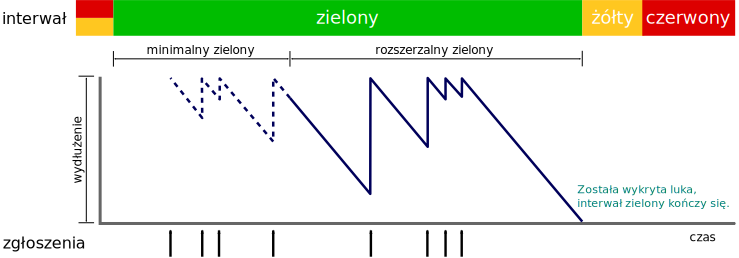
\includegraphics[width=0.7\textwidth]{img/signals-gap-out}
  \caption{Zakończenie sygnału zielonego przez wykrycie luki.}
\label{img:gap-out}
\end{figure}

Duże natężenie ruchu w danym potoku mogłoby powodować brak luk między
pojazdami i -- co za tym idzie~-- zbyt duże opóźnienia w obsłudze
pozostałych potoków. Aby ograniczyć z góry czas oczekiwania, określa
się maksymalny czas, w którym potok może otrzymywać sygnał zielony w
obecności zgłoszenia przeciwnego (patrz
rys. \ref{img:max-out}). Należy podkreślić, że w razie braku
zgłoszenia przeciwnego sygnał zielony będzie nadawany tak długo aż nie
nastąpi wykrycie luki.
\begin{figure}[ht] \centering
  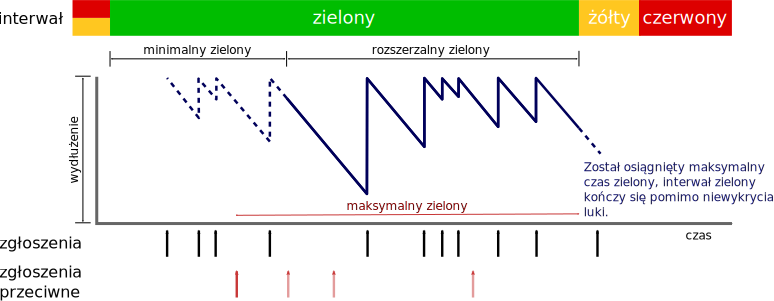
\includegraphics[width=0.7\textwidth]{img/signals-max-out}
  \caption{Zakończenie sygnału zielonego przez wykorzystanie
maksymalnego czasu.}
\label{img:max-out}
\end{figure}

\paragraph{Potoki pieszych} Tak jak w przypadku pojazdów potok pieszy
otrzymuje sygnał zielony tylko w wyniku zgłoszonego
zapotrzebowania. Jednak jako, że ilościowa ocena poziomu
zapotrzebowania w przypadku ruchu pieszych jest trudna technicznie,
przyjmujemy stałą długość interwału zielonego.

\subsection{Opis funkcjonowania sygnalizacji na poziomie pojedynczej
fazy}

Podstawowym elementem opisu fazy jest stwierdzenie, które potoki
wchodzą w jej skład. Faza może obejmować:
\begin{itemize}
  \item jeden lub więcej potoków pojazdów,
  \item jeden lub więcej potoków pieszych,
  \item kombinację pewnej liczby potoków pojazdów i pieszych.
\end{itemize}
\begin{figure}[h] \centering \subfloat[Faza wyłącznie dla pojazdów]{
    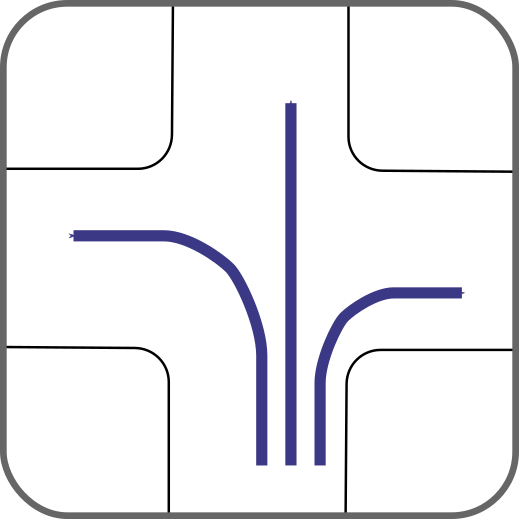
\includegraphics[width=0.27\textwidth]{img/signals-phase-example-1}
} \hfill \subfloat[Faza dla pojazdów oraz pieszych]{
    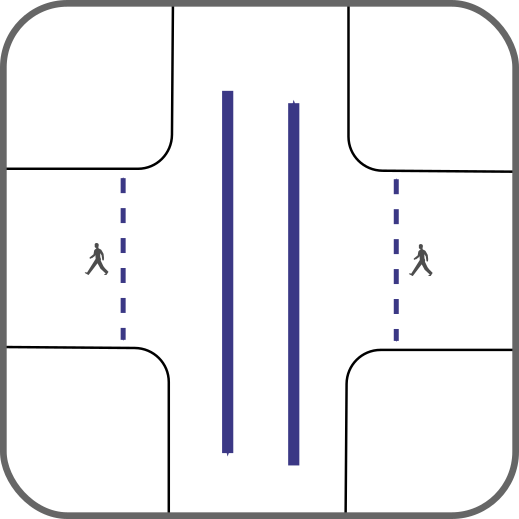
\includegraphics[width=0.27\textwidth]{img/signals-phase-example-2}
} \hfill \subfloat[Faza wyłącznie dla pieszych \ang{pedestrian
scramble, X~crossing}]{
    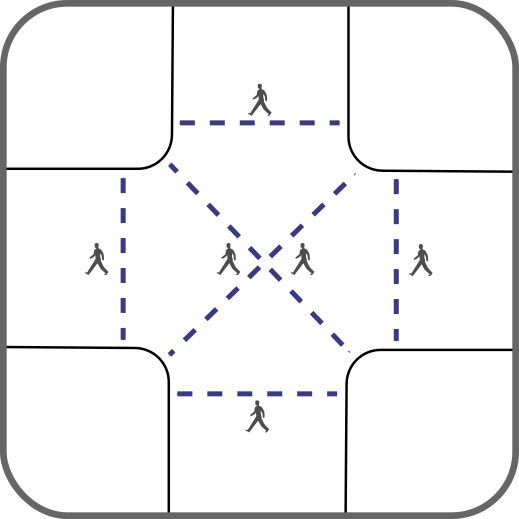
\includegraphics[width=0.27\textwidth]{img/signals-phase-example-3}
}
  \caption{Przykładowe fazy}
\end{figure}

Zauważmy, że choć już w opisie na poziomie potoku zaszła konieczność
zdefiniowania czasu maksymalnego, to powinien być on uważany za
właściwość fazy. Ustalenie różnych czasów maksymalnych dla różnych
potoków obniżałoby jedynie wydajność skrzyżowania w nieuzasadniony
sposób.

Dla faz jednopotokowych nie ma potrzeby podejmowania na tym etapie
żadnych dodatkowych decyzji projektowych, gdyż opis funkcjonowania
takiej fazy jest tożsamy z opisem funkcjonowania jej jedynego
potoku. Charakterystyka faz składających się z wielu potoków może być
bardziej złożona, jako że dopuszczają one większą liczbę możliwych
scenariuszy. Dotyczą one sytuacji, w których okres aktywności jednego
z potoków mógłby być różny od okresu aktywności fazy.

\paragraph{Zgłoszenia późne} Zgłoszeniami późnymi nazywany zgłoszenia
od zgłoszenia od potoków nieaktywnych, które otrzymano już po tym, gdy
faza stała się aktywna. Po pierwsze można uznać, że zostaną obsłużone
dopiero w następnym cyklu sygnalizacji (w takim wypadku traktowane są
tak samo jak zgłoszenia przeciwne). Drugą możliwoscią jest
obsługiwanie takich zgłoszeń w bieżącym cyklu, o ile nie spowoduje to
przekroczenia maksymalnej długości sygnału zielonego.
\begin{figure}[ht]
  \centering
  \subfloat[Opcja podtrzymania wyłączona]{
    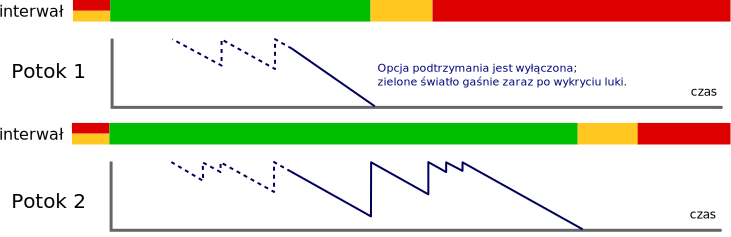
\includegraphics[width=0.8\textwidth]{img/signals-hold-1}
  }\\\vspace{1cm}
  \subfloat[Opcja podtrzymania włączona]{
    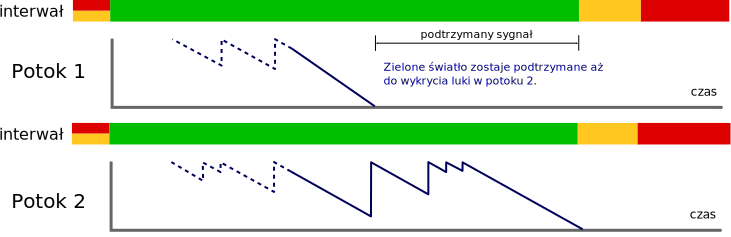
\includegraphics[width=0.8\textwidth]{img/signals-hold-2}
  }
  \caption{Opcja podtrzymania sygnału dla fazy dwupotokowej.}
  \label{img:signals-hold}
\end{figure}
\paragraph{Podtrzymanie} Innym elementem projektu wielopotokowej fazy
jest ustalenie zachowania się systemu w przypadku, gdy w jednym z
aktywnych potoków wykryta została luka, w innym zaś mamy do czynienia
z ciągłym zapotrzebowaniem. Możemy nie podejmować żadnego specjalnego
działania tj. wyłączyć sygnał zielony dla potoku, w którym czujnik
wykrył lukę.  Można w takim przypadku zastosować procedurę
\emph{podtrzymania sygnału} \ang{hold}. Polega ona na wydłużeniu
sygnału aż do momentu, w którym zakończą się sygnały zielone dla
pozostałych potoków (rys. \ref{img:signals-hold}).

\subsection{Opis funkcjonowania sygnalizacji dla cyklu} Opis cyklu
zawiera przede wszystkim informację o kolejności wchodzących w jego
skład faz.
\begin{figure}[h] \centering
  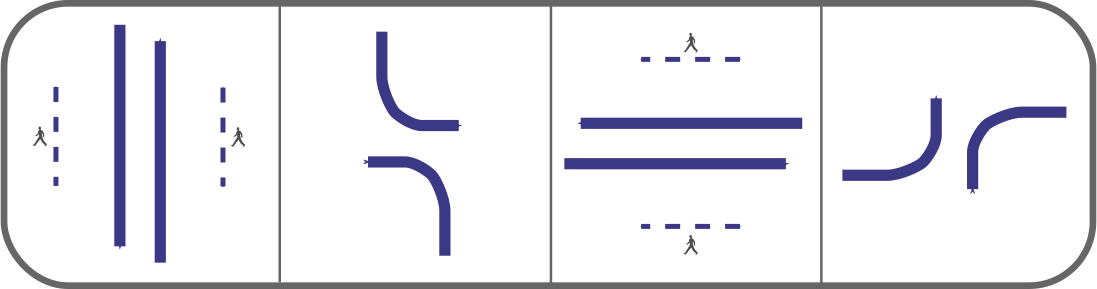
\includegraphics[width=0.7\textwidth]{img/signals-cycle-example}
  \caption{Przykładowy cykl}
\end{figure}

Jedyną dodatkową decyzją pozostającą do podjęcia na tym etapie jest
zachowanie się sygnalizacji w przypadku braku zgłoszeń tj. w
\emph{stanie spoczynku} \ang{rest}. Stosowane są dwa rozwiązania. Po
pierwsze wszystkie sygnalizatory mogą wyświetlać sygnał czerwony
\ang{rest in red}. Po drugie można wybrać fazę domyślną, która będzie
aktywna w przypadku braku jakiegokolwiek zapotrzebowania.

\subsection{Podsumowanie}

W rozdziale zaprezentowany został kompozycjonalny sposób opisu
systemów sygnalizacji wzbudzanej. Na początku zdefiniowano zachowanie
się sygnalizacji dla pojedynczego potoku, następnie potoki zostały
złożone w fazy, a fazy -- w cykl. Na każdym etapach dokładamy
informacje specyfikujące sposób owego złożenia.
Tabela \label{tab:signal-layer-params} podsumowuje parametry zawarte w
poszczególnych warstwach opisu.

\todo{Zrobić, żeby było ładnie}
\begin{table}[ht] \centering
  \begin{tabular}{|r|p{8cm}|} \hline Potok ruchu & parametry
określające długości interwałów
    \begin{itemize}
      \item interwały przejściowe
      \item parametry decydujące o długości interwału zielonego
      \begin{itemize}
        \item minimalny zielony
        \item maksymalny zielony
        \item wydłużenie
      \end{itemize}
    \end{itemize} \\\hline Faza & potoki składające się na fazę \\ &
czas maksymalny \\ & obsługa późnych zgłoszeń \\ & podtrzymywanie
sygnału zielonego \\\hline Cykl & fazy wchodzące w skład cyklu i ich
kolejność \\ & zachowanie w stanie spoczynku\\\hline
  \end{tabular}
  \caption{Parametry definiowane przez poszczególne warstwy opisu
systemu sygnalizacji.}  \ref{tab:signal-layer-params}
\end{table}

\chapter{Automaty czasowe}
\label{c:ta} Automaty czasowe są teoretycznym narzędziem
umożliwiającym modelowanie i weryfikację systemów czasu
rzeczywistego. Po zdefiniowaniu ich przez Alura i Dilla nie tylko
stały się popularnym obszarem badań teoretyków, lecz były także
stosowane w praktycznych problemach weryfikacyjnych.

\section{Automaty czasowe} Wersja formalizmu automatów czasowych
przedstawiona w niniejszym rozdziale pochodzi od Henzingera i
in.\cite{henz-94}. Jej teoretyczna siła wyrazu jest identyczna z siłą
wyrazu automatów w wersji Alura i Dilla, natomiast jest ona
wygodniejsza do praktycznego modelowania systemów.

Automat czasowy jest zwykłym automatem skończonym rozszerzonym o
zestaw zmiennych rzeczywistych nazywanych zegarami.  Stanem takie
automatu będziemy nazywali parę opisującą wierzchołek (tj. stan
odpowiedniego automatu skończonego), w którym znajduje się automat,
oraz wartościowanie zegarów. W stanie początkowym wartości wszystkich
zegarów są wyzerowane, natomiast w czasie jego działania wszystkie
zwiększają swoją wartość w tym samym tempie. Przyrost wartości zegarów
modeluje upływ czasu.

Aby móc modelować systemy o pożądanych własnościach, możemy nakładać
pewne dodatkowe warunki na tranzycje oraz wierzchołki, a także
wykonywać pewne operacje na zegarach. Każdej tranzycji możemy
przypisać wyrażenie opisujące wartościowanie zegarów, przy którym jej
wykonanie jest dozwolone. Analogiczne ograniczenia dla wierzchołków
nazywane są \emph{niezmiennikami}. Poprawne są tylko te stany automatu
czasowego, w których wartościowanie zegarów spełnia niezmiennik danego
wierzchołka.


\subsection{Formalna definicja} Przyjmijmy, że mamy skończony zbiór
$\mathcal{C}$ zmiennych rzeczywistych (zegarów) oraz skończony alfabet
$\Sigma$ (akcji).

\begin{definition}[Ograniczenie zegarowe] Ograniczeniem zegarowym
nazywamy koniunkcję formuł o postaci $x \sim n$ bądź $x - y \sim n$,
gdzie $x, y \in \mathcal{C}$, $n \in \mathbf{N}$, natomiast $\sim$
jest jedną spośród relacji $=, \le, \leq, \ge, \geq$.
\end{definition}
Zbiór ograniczeń zegarowych nad $\mathcal{C}$ będziemy oznaczali przez
$\mathcal{B}(\mathcal{C})$.

\begin{definition}[Automat czasowy] Automat czasowy jest $\mathcal{A}$
jest krotką $\langle N, l_0, E, I\rangle$, gdzie
  \begin{itemize}
    \item $N$ jest skończonym zbiorem wierzchołków,
    \item $l_0$ jest wierzchołkiem początkowym,
    \item $E \subseteq N \times \mathcal{B}(\mathcal{C}) \times \Sigma
    \times 2^{\mathcal{C}} \times N$ jest zbiorem krawędzi
    \item $I: N \mapsto \mathcal{B}(\mathcal{C})$ jest funkcją
    przypisującą wierzchołkom ich niezmienniki
  \end{itemize}
\end{definition}
Zamiast $\langle l, g, a, r, l' \rangle \in E$ będziemy pisali $l
\stackrel{g, a, r}{\longrightarrow} l'$. Zapis taki oznacza tranzycję
$a$ prowadzącą z wierzchołka $l$ do wierzchołka $l'$, którą można
wykonać przy wartościowaniu zegarów spełniającym ograniczenie $g$ i
przypisującą $0$ wszystkim zegarom z $r$.


Tak zdefiniowany automat czasowy rozumiemy jako
system przejść, w którym można wykonywać dwa rodzaje tranzycji:
\begin{description}
  \item[opóźnienie] polega na zwiększeniu wartości wszystkich zegarów
  o pewną liczbę rzeczywistą; intuicyjnie, jest to przebywanie przez
  jakiś czas w wierzchołku
  \item[wykonanie akcji] polega na przejściu do innego wierzchołka
  zgodnie z wybraną tranzycją; wykonanie akcji nie jest związane z
  upływem czasu (zmiana wartościowania zegarów może wynikać jedynie ze
  zresetowania niektórych z nich)
\end{description}
Formalnie ujmuje to poniższa definicja.
\begin{definition}[Semantyka operacyjna automatu czasowego] Semantyką
  automatu czasowego jest system przejść, którego stany są parami
$\langle l, u \rangle$ a przejścia spełniają następujące reguły:
  \begin{itemize}
    \item $\pair{l}{u} \stackrel{d}{\longrightarrow} \pair{l}{u+d}$
    jeśli $u \vdash I(l)$ oraz $(u+d) \vdash I(l)$ dla pewnego $d \in
    \mathbf{R}^{+}$
    \item $\pair{l}{u} \stackrel{a}{\longrightarrow} \pair{l'}{u'}$,
    jeśli $l \stackrel{g, a, r}{\longrightarrow} l', u \vdash g, u' =
    [r \mapsto 0]u$ oraz $u' \in I(l')$
  \end{itemize}
\end{definition}

\subsection{Problemy weryfikacyjne}

\section{UPPAAL}

\upp\ jest zestawem narzędzi pozwalającym na modelowanie systemów czasu
rzeczywistego przy pomocy automatów czasowych, ich symulację a także
weryfikację ich własności. Rozwijają go wspólnie Uniwersytet w Uppsali
oraz Uniwersytet w Aalborg. Pierwsza wersja narzędzia została wydana w roku
1995 \cite{lpw:fct95}.

\upp\ był wielokrotnie wykorzystywany w weryfikacji rzeczywistych
systemów: od protokołów komunikacyjnych po aplikacje multimedialne
(m.in. \cite{lp:prfts97}, \cite{lpw:tacas98},
\cite{DBLP:conf/icfem/BordbarO03},
\cite{Ravn:2011:MVW:1987389.1987431}). Był jednym z głównym narzędzi
stosowanych w -- prowadzonym przez konsorcjum europejskich
uniwersytetów i przedsiębiorstw -- projekcie \textsc{Ametist}, mającym
na celu rozwój przemysłowych metod weryfikacji systemów czasu
rzeczywistego \cite{AMETISTfinal}.

\subsection{Modelowanie}
Modelowanie w \upp-u polega nie tyle na tworzeniu jednego automatu
czasowego, lecz projektowaniu \emph{szablonów} automatów, których
instancje (nazywane procesami) tworzą model całego systemu. Dzięki
temu model podzielić na logiczne części o ściśle określonych
odpowiedzialnościach.

Model projektuje się przy pomocy prostego graficznego interfejsu
użytkownika (patrz rys.~\ref{img:uppaal-gui}). Wbudowany w aplikację
symulator pozwala na szybkie zapoznanie się z funkcjonowaniem systemu,
a także ułatwia przeglądanie kontrprzykładów dostarczanych przez
weryfikator. Co ważne, symulator pokazuje nie konkretne stany systemu,
a stany symboliczne (strefy). Przydatną funkcją jest także generacja
diagramu komunikacji procesów trakcie symulacji
(rys.~\ref{img:uppaal-msc}).
\begin{figure}[ht]
  \centering
  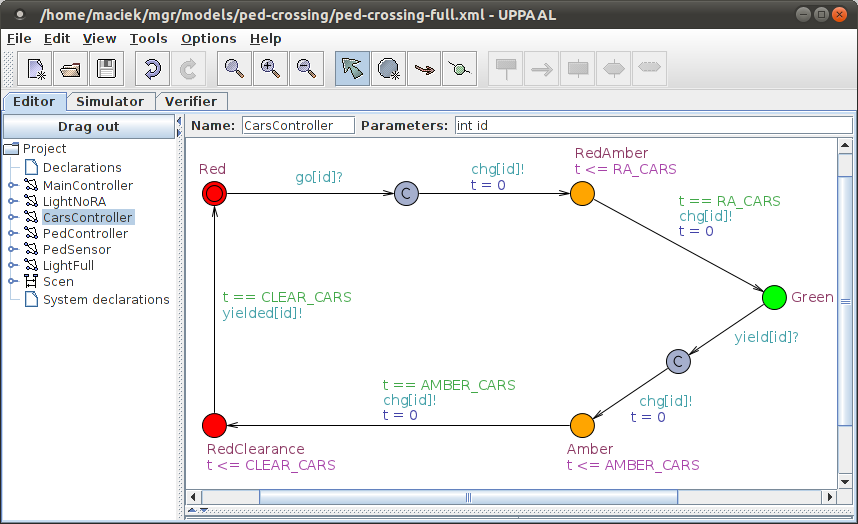
\includegraphics[width=0.9\textwidth]{img/uppaal-editor.png}
  \caption{Interfejs edytora szablonów procesów.}
  \label{img:uppaal-gui}
\end{figure}

\begin{figure}[ht]
  \centering
  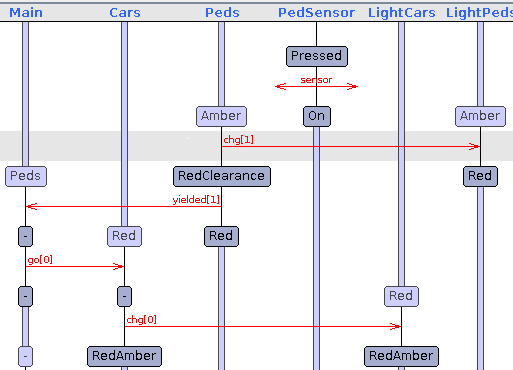
\includegraphics[width=0.9\textwidth]{img/uppaal-msc.png}
  \caption{Generowany przez symulator \upp-a diagram komunikacji
    procesów \ang{message sequence chart}.}
  \label{img:uppaal-msc}
\end{figure}

Autorzy \upp-a rozszerzyli podstawową definicję automatów czasowych o
dodatkowe konstrukcje \cite{by-lncs04}. Większość nie zwiększa siły
wyrazu formalizmu, a jedynie ułatwia modelowanie bardziej złożonych
systemów.  Poniżej opisane zostaną najważniejsze rozszerzenia.

\paragraph{Komunikacja} Możliwość modelowania przy pomocy sieci
automatów czasowych wiąże się z koniecznością wprowadzenia mechanizmu
komunikacji pomiędzy poszczególnymi procesami. W \upp-u jest ona
realizowana poprzez synchronizację na kanałach komunikacyjnych.
\todo{dopisać}.
\todo{broadcast}.

\paragraph{Zmienne całkowitoliczbowe} Obok zmiennych zegarowych
użytkownik może deklarować także zmienne całkowitoliczbowe oraz
tablice. Wyrażeń na nich można używać w ograniczeniach na krawędziach
oraz niezmiennikach wierzchołków. Przypisania na zmienne wykonywane są
w trakcie przejścia (analogicznie do resetowania zegarów).

\paragraph{Wierzchołki pilne oraz przymusowe} Wprowadzono możliwość
dodatkowego oznaczenia wierzchołków automatów jako \emph{pilne}
\ang{urgent} bądź \emph{przymusowe} \ang{committed}.

Jeśli automat jest w wierzchołku pilnym, nie może wykonać opóźnienia
(żaden czas nie może upłynąć). Jest to równoważne zadeklarowaniu
dodatkowego zegara $t$, który będzie resetowany na wszystkich
krawędziach wchodzących do danego wierzchołka oraz nadaniu mu $t \leq
0$(\ref{img:uppaal-urgent}). Jako pilne mogą być oznaczone także
kanały komunikacyjne; procesy muszą się zsynchronizować na takim
kanale tak szybko jak będzie to możliwe.

\begin{figure}[ht]
  \centering
  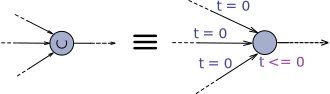
\includegraphics[width=.8\textwidth]{img/uppaal-urgent}
  \caption{Wierzchołek pilny i równoważny mu wierzchołek z dodatkowym
    zegarem}
  \label{img:uppaal-urgent}
\end{figure}

Jeszcze mocniejszą własność mają wierzchołki przymusowe. Są to
wierzchołki pilne, z których przejście należy wykonać tak szybko jak
to możliwe. Jeśli któryś z procesów jest w wierzchołku przymusowym,
system nie może wykonać przejścia z wierzchołka nieprzymusowego.
Wierzchołki przymusowe są bardzo przydatne np. w modelowaniu atomowych
ciągów komunikacji pomiędzy wieloma procesami.

\subsection{Weryfikacja}

Weryfikator \upp-a pozwala na dowodzenie własności opisywanych przez
podzbiór języka TCTL \cite{acd:mc}. Poprawne są wszystkie formuły
następujących postaci \cite{by-lncs04}:
\begin{itemize}
  \item \texttt{A[] $\varphi$} -- ,,zawsze $\varphi$'' (bezpieczeństwo),
  \item \texttt{E<> $\varphi$} -- ,,być może kiedyś $\varphi$''
  (osiągalność),
  \item \texttt{A<> $\varphi$} -- ,,zawsze kiedyś $\varphi$'',
  \item \texttt{E[] $\varphi$} -- ,,być może zawsze $\varphi$''
  \item \texttt{$\varphi$ --> $\psi$}\footnote{W czystym TCTL własność
    ta zostałaby zapisana następująco: \texttt{A[]
      ($\varphi\rightarrow$ A<> $\psi)$}} -- ,,$\varphi$ zawsze
  prowadzi do $\psi$'' (żywotność),
\end{itemize}
gdzie $\varphi$ i $\psi$ są własnościami stanu tj. predykatami
dotyczącymi wierzchołków oraz zmiennych liczbowych i zegarów.

Semantykę powyższych formuł oparta jest na rozwinięciu kolejnych
przejść w potencjalnie nieskończone drzewo. Litery \texttt{A} i
\texttt{E} w formułach wprowadzają kwantyfikację po ścieżkach:
\texttt{A} oznacza, że dana własność ma być spełniona dla wszystkich
ścieżek, zaś \texttt{E} -- dla co najmniej jednej. Symbole
\texttt{[]} oraz \texttt{<>} kwantyfikują stany na pojedynczej
ścieżce: \texttt{[]} mówi, że własność ma być spełniona dla wszystkich
stanach na ścieżce, zaś \texttt{<>} -- dla co najmniej jednego. 

 \begin{figure}[ht]
   \centering
   \subfloat[{\texttt{A[] $\varphi$}}]{
     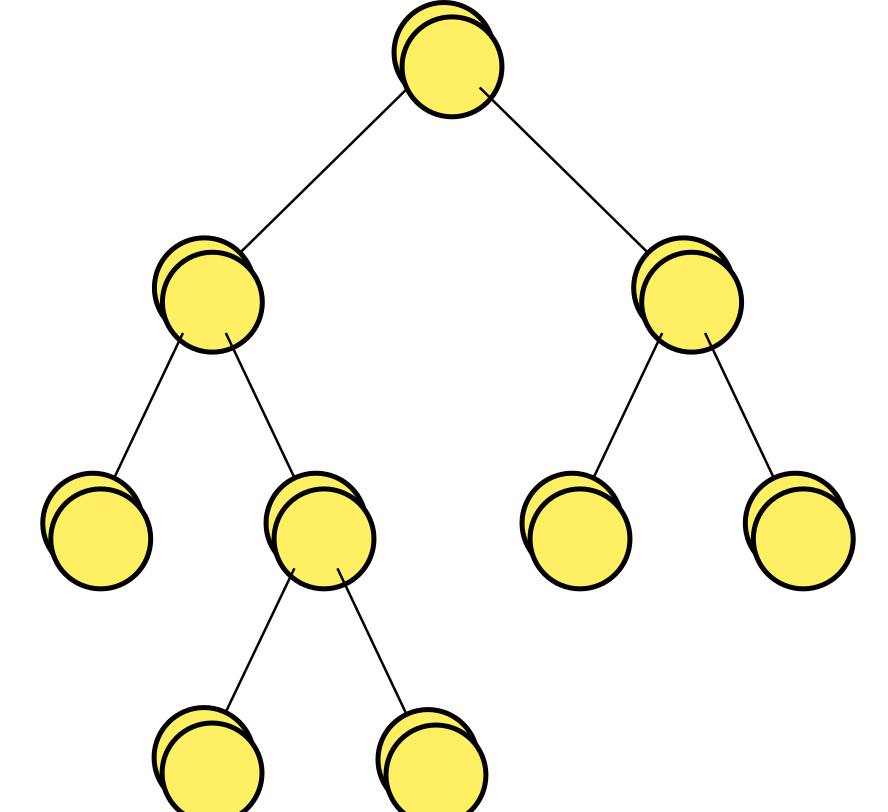
\includegraphics[width=0.3\textwidth]{img/uppaal-tctl-1}
   }
   \subfloat[\texttt{A<> $\varphi$}]{
     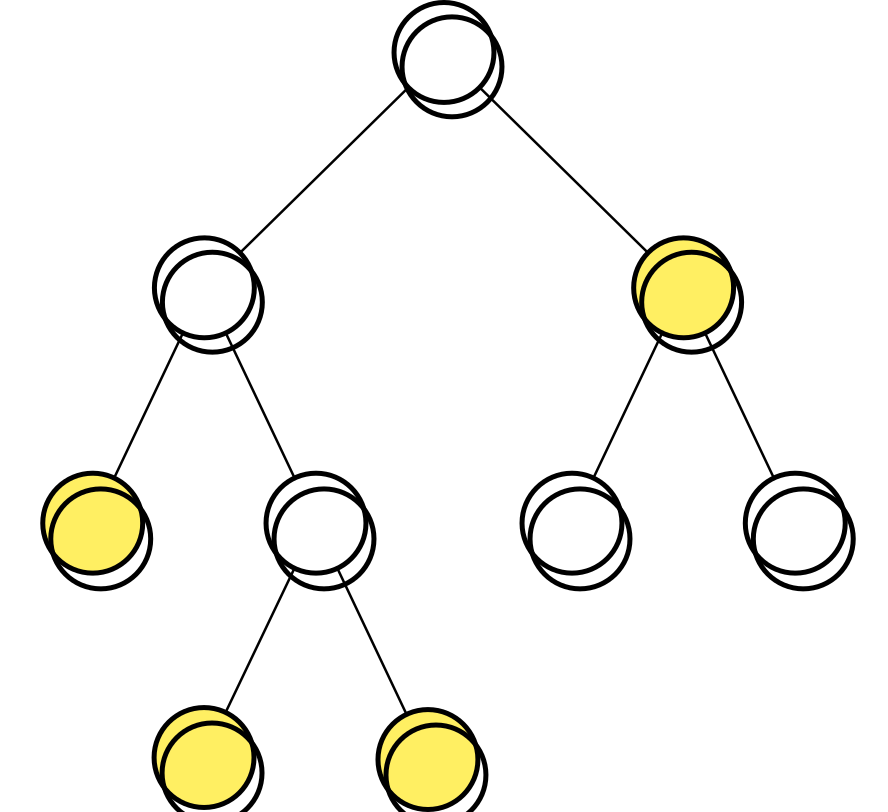
\includegraphics[width=0.3\textwidth]{img/uppaal-tctl-2}
   }\\
   \subfloat[\texttt{E[] $\varphi$}]{
     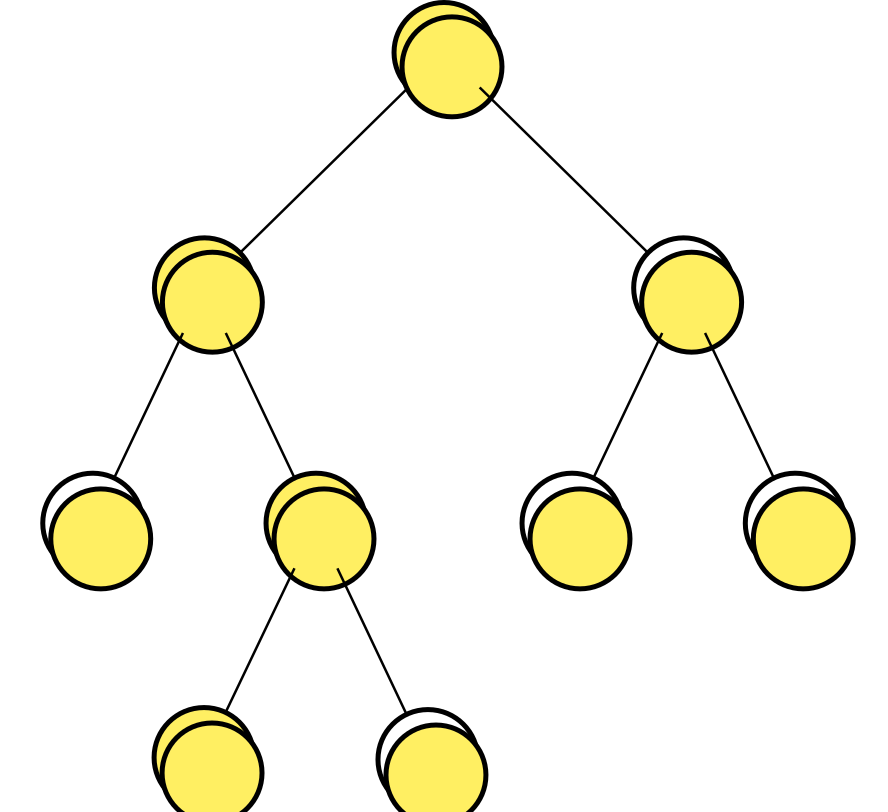
\includegraphics[width=0.3\textwidth]{img/uppaal-tctl-3}
   }
   \subfloat[\texttt{E<> $\varphi$}]{
     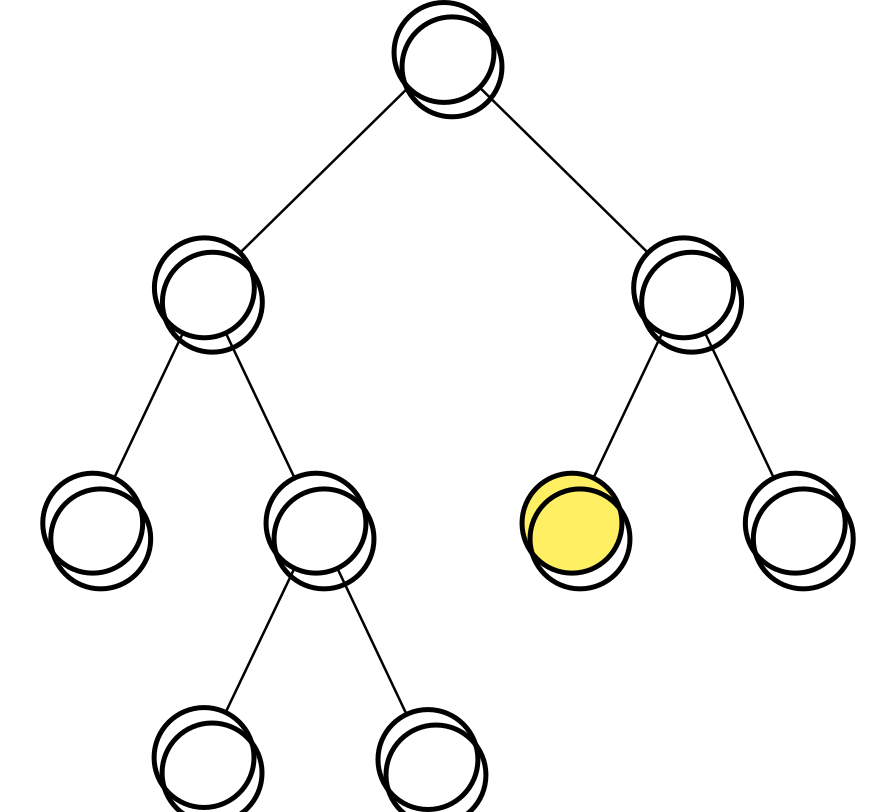
\includegraphics[width=0.3\textwidth]{img/uppaal-tctl-4}
   }
   \subfloat[\texttt{$\varphi$ --> $\psi$}]{
     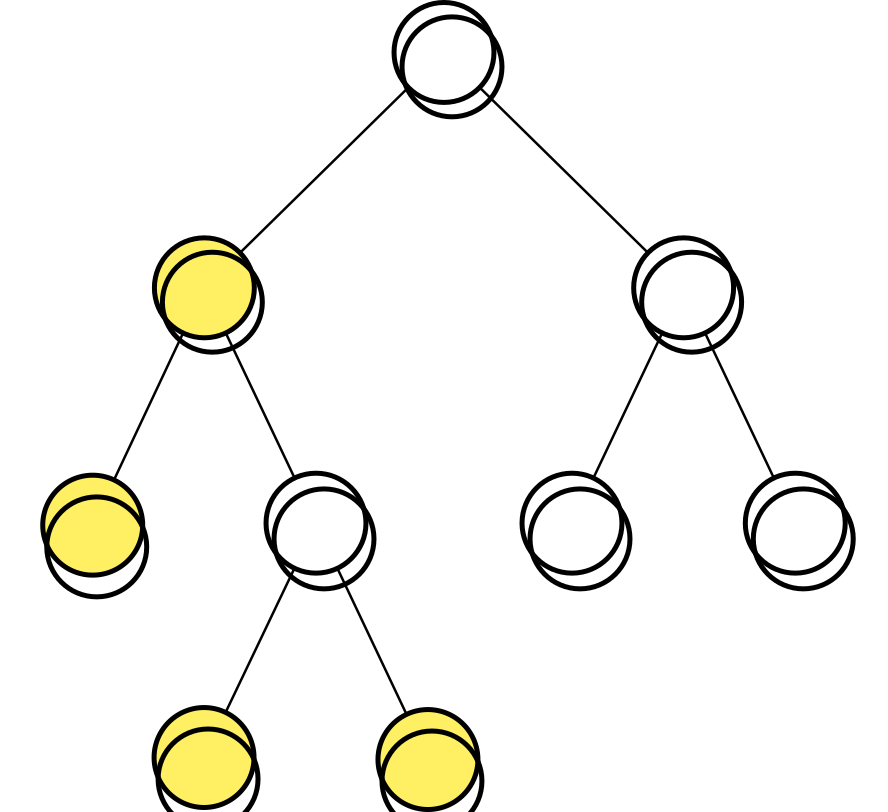
\includegraphics[width=0.3\textwidth]{img/uppaal-tctl-5}
   }
   \caption{Własności TCTL}
   \label{img:tctl-props}
 \end{figure}
O deadlocku.
Dodatkowo można takżę

 
\chapter{Język modelowania}



\bibliography{bib.bib}{}
\bibliographystyle{plalpha}


% \begin{thebibliography}{99}
% \addcontentsline{toc}{chapter}{Bibliografia}

% % http://ops.fhwa.dot.gov/publications/fhwahop06006/form_dot_1700.htm
% \bibitem[FHWA06]{handbook} Robert L. Gordon, Warren Tighe,
% \textit{Traffic Control Systems Handbook}, Federal Highway
% Administration, 2006.

% % http://ops.fhwa.dot.gov/publications/fhwahop08024/doc_page.htm
% \bibitem[FHWA08]{timing} Peter Koonce i in., \textit{Traffic Signal
%   Timing Manual}, Federal Highway Administration, 2008.

% \end{thebibliography}

\end{document}

%%% Local Variables:
%%% mode: latex
%%% TeX-master: t
%%% coding: utf-8
%%% eval: (auto-fill-mode 1)
%%% End:

% LocalWords:  stałoczasowa
